\documentclass[12pt,a3paper]{article}
\usepackage{better_poster}


% ---- fill in from here

% authors
\title{A title for the robot}
\author{A project in IN5590 by your\_full\_name E-mail: username@ifi.uio.no }

% type of poster: [exp]erimental results, [methods], [theory]
% Disclaimer: the original classification had "study" and "intervention" as separate categories. I group them under experimental results.
\newcommand\postertype{exp} % [exp],[methods],[theory]

\begin{document}

% main point of your study
\makefinding{
\textbf{Name of robot}.
}


% \makemain{
% }{

% }


% the main text of your poster goes here
\makemain{
    % you can have 1 or 2 columns
    \raggedcolumns
    \begin{multicols}{2}
        \section{Intro}
        Write a couple of sentences about your prototype here.
        \begin{itemize}
        \setlength\itemsep{0.1em}
            \item Enlist your goals from assignment 4.
        \end{itemize}
        
        Include the image from \textit{task 2} in the assignment. Additionally, include
        images from previous assignments that you see fit. You can choose whether you'd like to include 
        them in the \textit{extra column} or in the text.
        \section{Tools}
        Describe the tools used here. 

        Enlist most important components. E.g:
        \begin{itemize}
        \setlength\itemsep{0.1em}
            \item Dynamixel AX12
            \item Pneumatic cylinders
            \item Arduino
        \end{itemize}

        Include a description on the software that is interesting. Like language, libraries used, algorithms etc. 
        
    % this determines where your columns will be separated
    \columnbreak

        \section{Conclusion}

        Write a paragraph about how far you came in achieving the goals.

        Write a paragraph on \textit{Future work}. What would improve the robot? What could you do differently? 
    
    \end{multicols}
}
% If you have extra figures or data to show
\makeextracolumn{
    Add your things here
    
    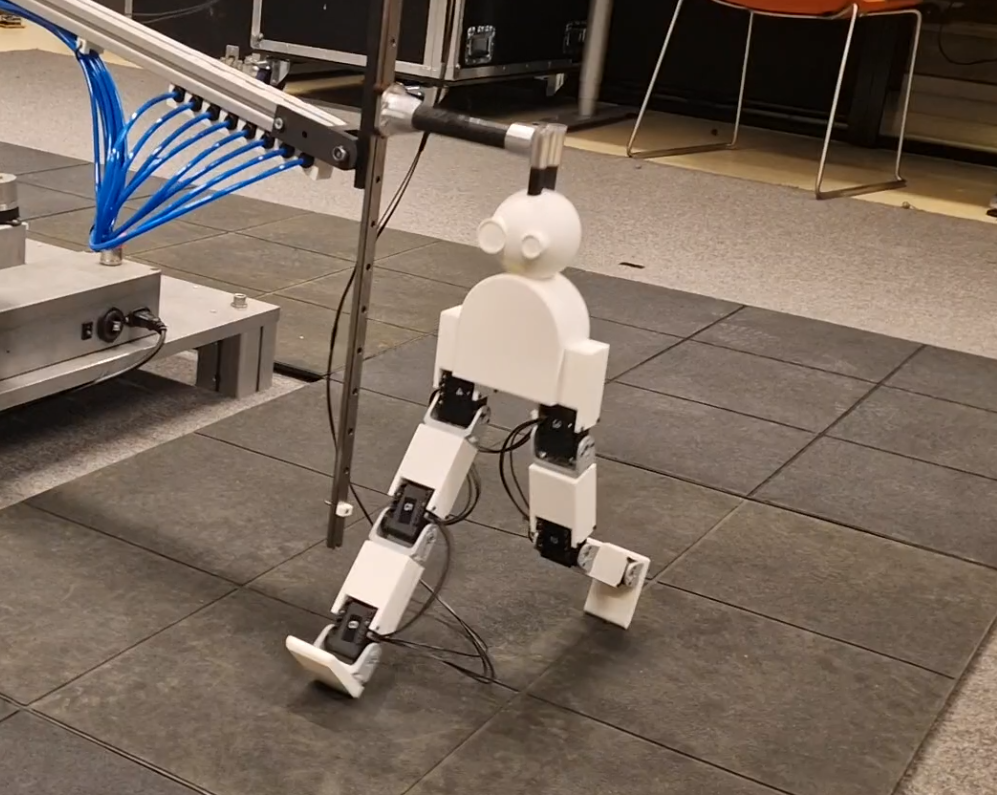
\includegraphics[width=0.5\linewidth]{2.png}

    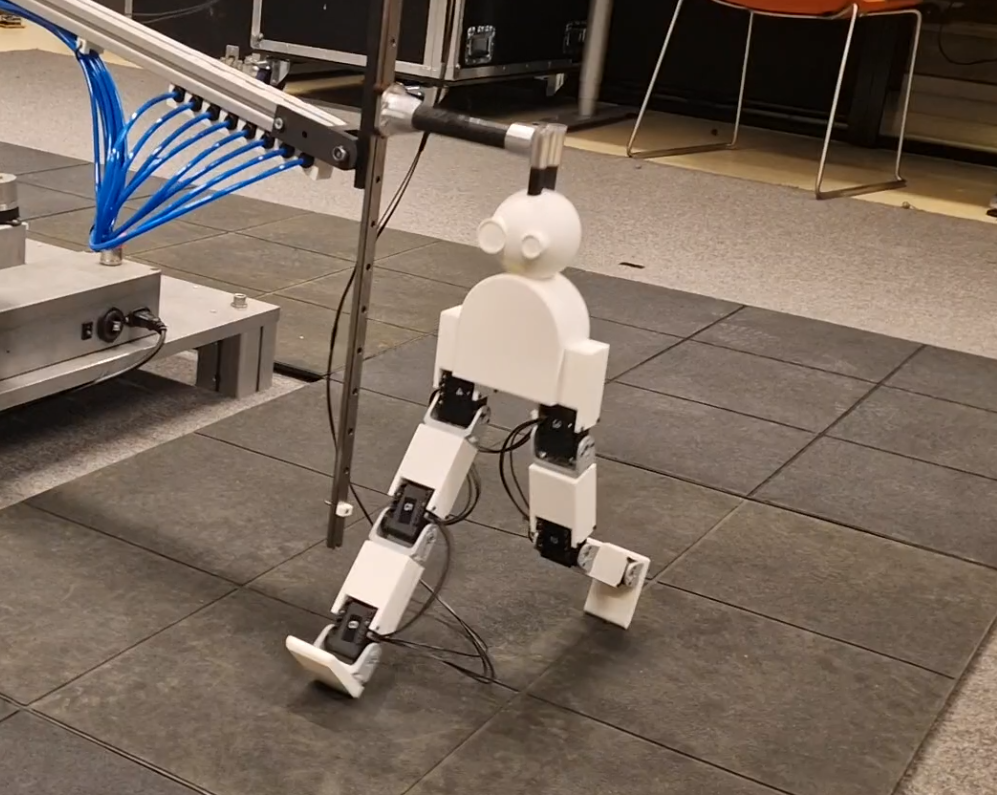
\includegraphics[width=0.5\linewidth]{2.png}
    
    \begin{itemize}
    \setlength\itemsep{0.1em}
        \item Stuff you don't want to forget
        \item But is not essential
    \end{itemize}
}

% footer
% generate qr code from https://www.qr-code-generator.com/ and replace qr_code.png
% default: barcode on the left
\makealtfooter{images/uni_logo.pdf}{images/qr-code.png}

% replace with this like for barcode on the right
%\makealtfooter{images/uni_logo.png}{images/qr-code.png}
 
\end{document}
